\documentclass{article}

\usepackage{url} 

\usepackage{pdfpages}
\usepackage{lastpage}
\usepackage{fancyhdr}
\usepackage{ngerman}
\usepackage{listings}

\usepackage{floatrow}
\usepackage[tableposition=top]{caption}
\floatsetup[table]{capposition=top}

\usepackage{amsmath, amssymb}

\usepackage[utf8]{inputenc}


\usepackage[numbib]{tocbibind}



\newcommand\twodigits[1]{%
   \ifnum#1<10 0#1\else #1\fi
}



\lhead{Silbercoulombmeter}
\rhead{23. Oktober 2020\\T. Maier, J. Winkler}
%\cfoot{\twodigits{\thepage}~/ \pageref{LastPage}}
\cfoot{{\thepage}~/ \pageref{LastPage}}

\newcommand{\as}{\alpha_\text{spez}}

\begin{document}

\parindent0cm

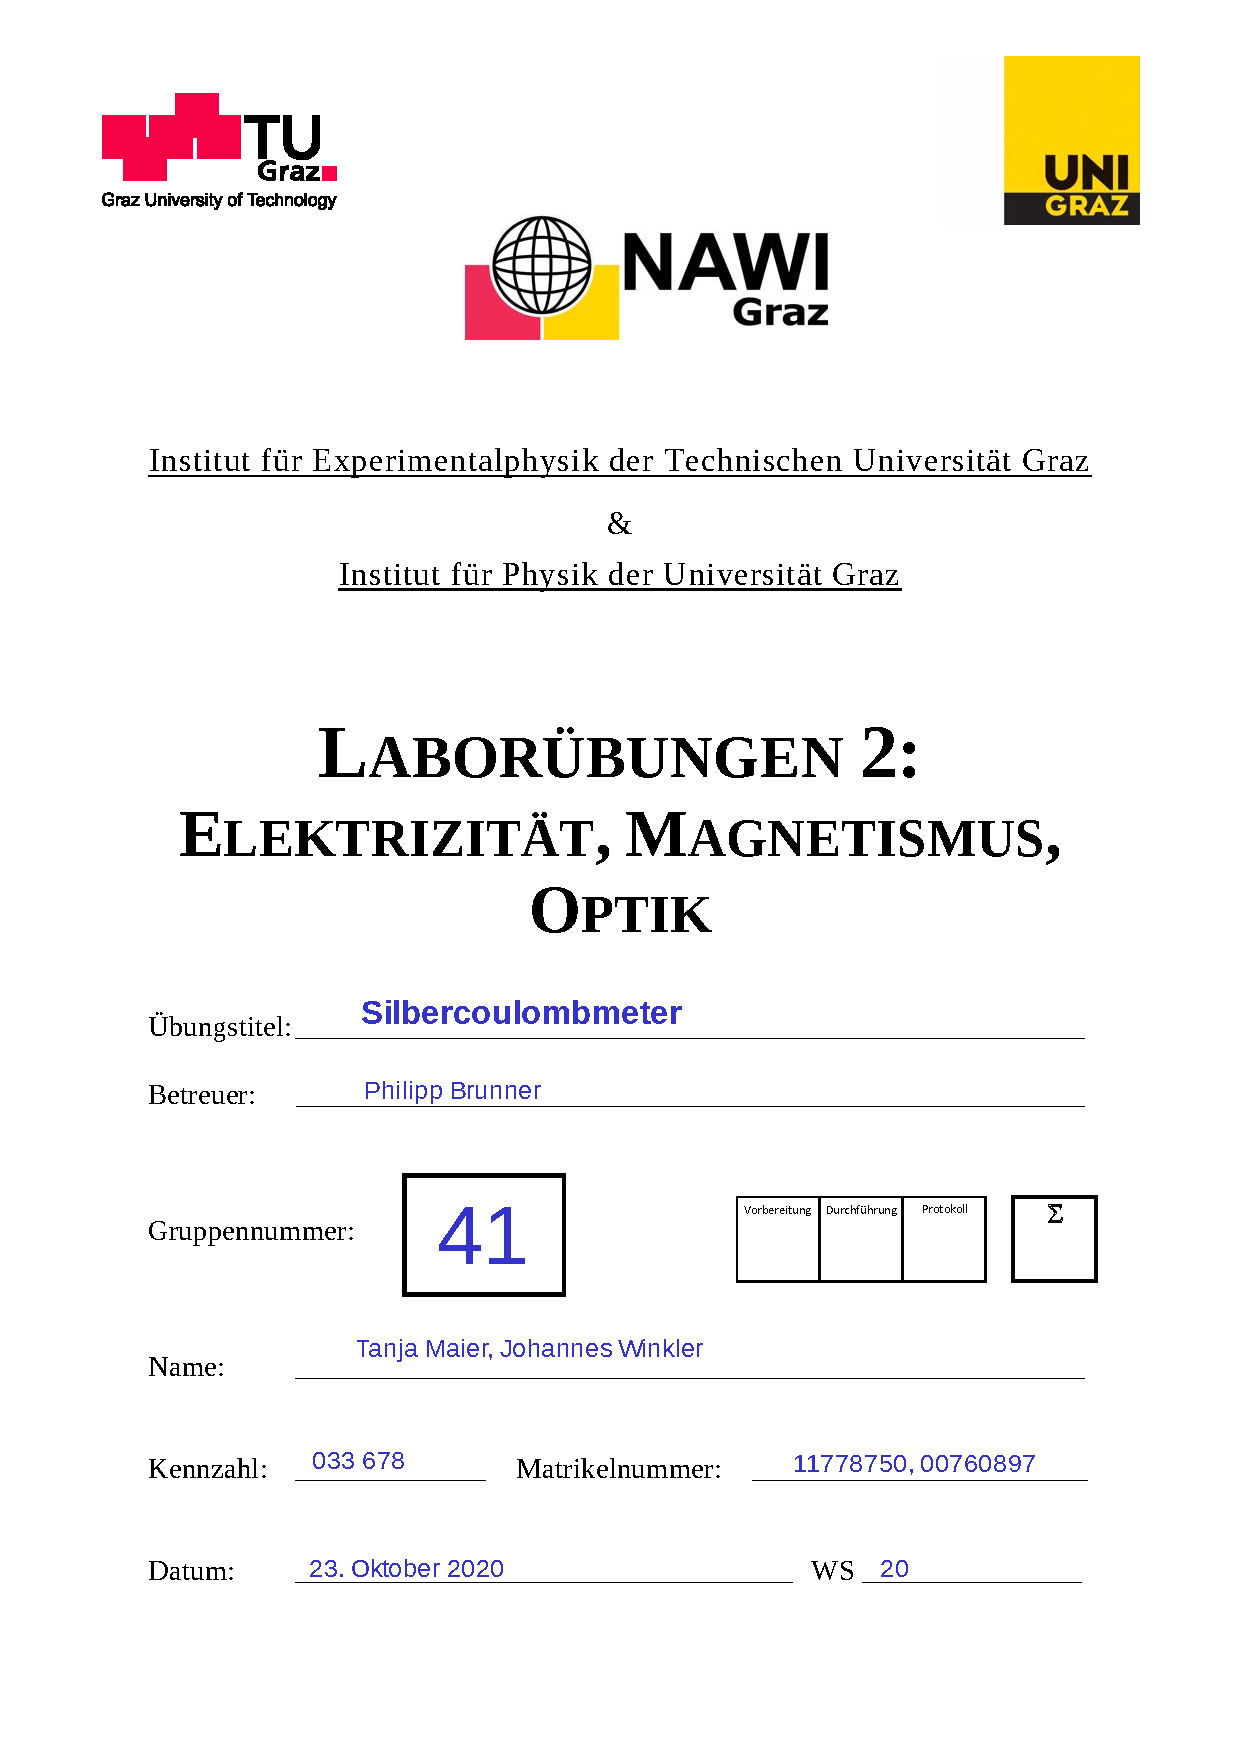
\includepdf{Deckblatt.pdf}


\pagestyle{fancy}

\section{Aufgabenstellung}

\paragraph{Silbercoulombmeter}
Berechnung der Faraday-Konstante mithilfe eines Silbercoulometers. Berechnung der Elementarladung.

\paragraph{Elektrolyse}
Bestimmung der Dichte der verd+nnten Schwefelsäure mithilfe eines Aräometers. Messung der bei der Elektrolyse entstehenden Wasserstoffmengen bei verschiedenen Stromstärken und Zeitdauern. Bestimmung der Faraday-Konstante, des elektrochemischen Äquivalents und der Elementarladung über die Masse des abgeschiedenen Wasserstoffes.





\section{Grundlagen und Versuchsaufbau}

Grundsätzlich versteht man unter Elektrolyse die chemische Zersetzung einer Flüssigkeit beim Durchgang eines Stromes. Stromleitende Flüssigkeiten nennt man Elektrolyt. Die Leitung in einem Elektrolyten erfolgt dabei über frei bewegliche Ionen im elektrischen Feld. Bei anliegen eines elektrischen Feldes, wandern die positiv geladen Kationen nur negativ geladenen Elektrode (Kathode), die negativ geladen Anionen zur positiv geladenen Elektrode (Anode). Die Kationen nehmen an der Kathode Elektronen auf und werden dadurch neutral. Die Anionen geben an der Anode Elektronen ab und werden ebenfalls neutral.



\begin{figure}[H]
\caption{Ionentransport im Elektrolyten im elektrischen Feld. $A$ Anode, $K$ Kathode.}
\label{fig:pic1}
{\centering
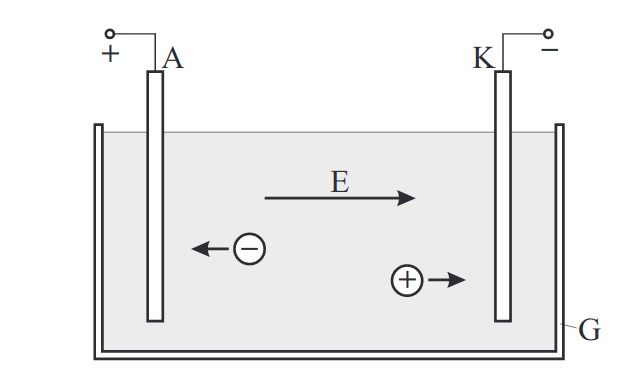
\includegraphics[scale=1.8]{pic1.png}}
\end{figure}

Bei einer Elektrolyse treten also an den beiden Elektroden chemische Vorgänge auf. Dabei gilt für die gesamt geflossene Elektrizitätsmenge
\begin{align}
q = n\cdot e \cdot z
\end{align}
wobei $n$ die Zahl der $z$-wertigen Ionen, $q$ die durch den Elektrolyten geflossene Elektrizitätsmenge und $e$ die Elementarladung ist.

Zur Bestimmung der Faraday-Konstante $F$ schickt man durch den Elektrolyten in einer Zeitspanne $t$ einen gemessenen Strom $I$ (und somit eine bekannte Elektrizitätsmenge $q$) und bestimmt die Menge $m$ eines an einer Elektrode abtransportierte Stoffmenge. Für ein z-wertiges Ion ergibt sich so das 1. Faraday'sche Gesetz
\begin{align}
q = I\cdot t = \frac{m}{M} \cdot F \cdot z
\end{align}



Die Stoffmenge der Elektrizitätsmenge durch einen Elektrolyten ist proportional zum Produkt von Stromstärke und Zeit.

Der Einfachheit wegen wählt man hierbei einen Elektrolyten, der ein stabiles Reaktionsprodukt ergibt, sodass durch Umformen leicht $F$ bestimmt werden kann. Umgekehrt kann man bei bekanntem $F$ auch leicht die Elektrizitätsmenge berechnen. Solche Apparaturen werden daher als Coulometer bezeichnet.

Unter Berücksichtigung des elektrochemischen Äquivalents $C$ (Stoffmenge, die bei der Elektrolyse mit einem Coulomb abgeschieden wird \cite{chemie}) gilt außerdem
\begin{align}
C = \frac{m_x}{z\cdot e} = \frac{m_x\cdot N_A}{z\cdot e \cdot N_A} = \frac{m_A}{z\cdot F}
\end{align}
Sowie auch das 2. Faraday'sche Gesetz: Die elektrochemischen Äquivalente zweier Stoffe verhalten sich gleich wie ihre chemischen Äquivalente.





\section{Geräteliste}

\begin{table}[H]
\caption{Liste der verwendeten Geräte}

\begin{tabular}{l|llll}
Bezeichnung & Hersteller & Gerätenummer & Unsicherheit \\
\hline
Lineal & & & $\pm 1~$mm \\
Thermometer & & & $\pm 1~^\circ$C \\
Amperemeter & & $\pm 2$~mA \\
Hoffmann'scher Apparat  & & \\
Stoppuhr & Apple & iPhone XS Max & $\pm 1~$s \\
Waage & Mettler P163 &  & $\pm 1~$mg \\
Netzteil & GW & GPR-3030 & 
\end{tabular}

\end{table}




\section{Durchführung und Messwerte}

\subsection{Silbercoulombmeter}
Der Versuch wird gemäß Abbildung \ref{fig:pic1} aufgebaut. Die aus Silber bestehenden Elektroden werden abgeschliffen und ausführlich gewogen. Danach werden sie in den Behälter gehängt und an den Stromkreis angeschlossen. Es gilt $I=100~$mA für $t=1800~$s. Nach einer halben Stunde werden die Elektroden aus dem Behälter genommen und erneut abgewogen.

\begin{table}[H]
\caption{Gewichter der Elektroden für Tanja Maier (TM) und Johannes Winkler (JW). Alle Gewichter haben eine Unsicherheit von $\pm 1~$mg.}

\begin{tabular}{l|ll}
Bezeichnung & TM & JW \\
\hline
Kathode vorher / g & 9.406 & 9.641 \\
Kathode nachher / g & 9.613 & 9.861 \\
Anode vorher / g & 6.756 & 9.639  \\
Anode nachher/ g & 6.237 & 9.486 \\
\end{tabular}

\end{table}



\subsection{Elektrolyse}
Zuerst wurde die Dichte der Schwefelsäure $\rho$ bestimmt. Die Raumtemperatur wurde vom Thermometer mit $T=22^\circ$ bzw $T=295.15$~K abgelesen. Die Elektrolyse wurde für $t=600~$s (bzw. 10 Minuten) bei $I=300~$mA bzw $I=400~$mA durchgeführt.


\begin{table}[H]
\caption{Daten für die Elektrolyse von Tanja Maier (TM) und Johannes Winkler (JW)}

\begin{tabular}{l|lll}
Bezeichnung & TM & JW & Unsicherheit \\
\hline
$\rho({\text{H}_2\text{SO}_4})$ / g/dm${}^3$ & 1110 & 1106 & $\pm 4$ \\
$t$ / s & 600 & 600 & $\pm 30$ \\
$p_{\text{Luft}}$ / hPa & 1016 & 1016 & $\pm 1$ \\
$p_{\text{Dampf}}$ / Pa & 2500 & 2500 & $\pm 100$ \\
$I$ / mA & 400 & 300 & $\pm 5$ \\
Höhe Anode / cm & 14.0 & 11.5 & $\pm 1.0$ \\
Höhe Kathode / cm & 24.0 & 18.5 & $\pm 1.0$ \\
Volumen Anode / ml & 16.4 & 11.4 & $\pm 0.4$ \\
Volumen Kathode / ml & 33.8 & 24.0 & $\pm 0.4$ \\
$T$ / ${}^\circ$C & 22 & 22 & $\pm 1$
\end{tabular}

\end{table}



\section{Auswertung}

\subsection{Silbercoulombmeter}
Beim Silbercoulombmeter wird für die Faraday-Konstante folgende Formeln benötigt.
\begin{align*}
F &= \frac{I\cdot t\cdot M}{m\cdot z} \\
\Delta F &= \frac{\Delta I\cdot t\cdot M}{m\cdot z} + \frac{I\cdot \Delta t\cdot M}{m\cdot z} +\frac{I\cdot t\cdot M}{m^2\cdot z}\cdot \Delta m
\end{align*}
Es gilt $z=1$ und $M=107.87~$g/mol laut \cite{silber}. Zusätzlich gilt $I=(100~\pm~5)~$mA und $t=(1800~\pm~30)~$s. Der Wert $m$ wird aus der Differenz der Elektroden abgelesen.

Für die Auswertung ergibt sich bei Tanja Maier
\begin{align*}
F_\text{Kathode} &= (94 \pm 47)~\text{kC/mol}\\
F_\text{Anode} &= (37 \pm 8)~\text{kC/mol} \\
e_\text{Kathode} &= (1.56 \pm 0.78)\cdot 10^{-19}~C \\
e_\text{Anode} &= (0.62 \pm 0.62)\cdot 10^{-19}~C  
\end{align*}

Bei den Messwerten von Johannes Winkler ergibt sich
\begin{align*}
F_\text{Kathode} &= (88 \pm 46)~\text{kC/mol}\\
F_\text{Anode} &= (127 \pm 91)~\text{kC/mol} \\
e_\text{Kathode} &= (1.5 \pm 0.8)\cdot 10^{-19}~C \\
e_\text{Anode} &= (2.1 \pm 2.1)\cdot 10^{-19}~C  
\end{align*}




\subsection{Elektrolyse}


Die Berechnung der Faraday Konstante wird mit der Formel
\begin{align}
F = \frac{I\cdot t\cdot R \cdot T}{z \cdot V \cdot (p_L +\rho \cdot g \cdot h - p_D)}
\end{align}
durchgeführt, wobei $p_L$ der Luftdruck, $p_D$ der Dampfdruck und $\rho$ die Dichte der Schwefelsäure ist.

Die Fehlerrechnung ist
\begin{align*}
\Delta F &= F\cdot \frac{\Delta T}{T} + F\cdot \frac{\Delta t}{t} + F\cdot \frac{\Delta I}{I} + F \cdot \frac{\Delta V}{V}  + F\cdot \frac{\Delta p_L + \Delta p_D + g\cdot (\Delta\rho \cdot h + \rho\cdot \Delta h)}{(p_L +\rho \cdot g \cdot h - p_D)}\\
\Delta F &= F\cdot \left(\frac{\Delta T}{T} + \frac{\Delta t}{t} + \frac{\Delta I}{I} + \frac{\Delta V}{V}  + \frac{\Delta p_L + \Delta p_D + g\cdot (\Delta\rho \cdot h + \rho\cdot \Delta h)}{(p_L +\rho \cdot g \cdot h - p_D)}\right)
\end{align*}


Insgesamt ergibt sich bei Tanja Maier
\begin{align*}
F_\text{Kathode} &= (86 \pm 7)~\text{kC/mol}\\
F_\text{Anode} &= (89 \pm 8)~\text{kC/mol} \\
e_\text{Kathode} &= (1.4 \pm 1.6)\cdot 10^{-19}~C \\
e_\text{Anode} &= (1.5 \pm 0.1)\cdot 10^{-19}~C  
\end{align*}

Insgesamt ergibt sich bei Johannes Winkler
\begin{align*}
F_\text{Kathode} &= (91 \pm 8)~\text{kC/mol}\\
F_\text{Anode} &= (97 \pm 10)~\text{kC/mol} \\
e_\text{Kathode} &= (1.5 \pm 1.1)\cdot 10^{-19}~C \\
e_\text{Anode} &= (1.6 \pm 0.2)\cdot 10^{-19}~C  
\end{align*}


\subsection{Elektrochemisches Äquivalent}

Für Sauerstoff ist die molare Masse laut \cite{equiv} 15.994 und für Wasserstoff 1.0074. Die im Versuch $H_2$ und $O_2$ Moleküle betrachtet wurden, verdoppelt sich die Masse entsprechend. Für die Berechnung ist die Faraday-Konstante nötig.

Es gilt
\begin{align*}
C &= \frac{m}{z\cdot F} \\
\Delta C &= \frac{m}{z\cdot F^2}\cdot \Delta F
\end{align*}
wobei wir hier die molare Masse $m$ als exakt annehmen. Die Wertigkeit für ein $H_2$ Molekül liegt entsprechend bei $z=2$ und bei einem $O_2$ Molekül bei $z=4$.

Für die Berechnung wurden die Faraday-Konstanten aus dem Hoffmann Versuch bei der Anode verwendet.

Es ergibt sich bei Tanja Maier
\begin{align*}
C_{O_2} = (0.090 \pm 0.008)~\text{mg}/\text{As} \\
C_{H_2} = (0.011 \pm 0.001)~\text{mg}/\text{As} 
\end{align*}

Es ergibt sich bei Johannes Winkler
\begin{align*}
C_{O_2} = (0.083 \pm 0.009)~\text{mg}/\text{As} \\
C_{H_2} = (0.010 \pm 0.001)~\text{mg}/\text{As} 
\end{align*}



\section{Diskussion}

Grundsätzlich  würde  die  Faraday-Konstante  beim  Silbercoulometer  mit  der Massendifferenz der Anode berechnet werden, da nicht der gesamte Silberniederschlag an der Kathode hängen bleibt und die Massendifferenz somit ein ungenaueres Maß wäre. In unserem Fall konnte jedoch ein passenderes Ergebnis mit der Kathode ermittelt werden und so wurden beide Werte berücksichtigt.Da beide Werte jedoch einen sehr großen Fehler aufweisen, lässt sich an der Genauigkeit dieses Versuchs zweifeln. Grund für die sehr große Ungenauigkeit ist beispielsweise  die  starke  Schwankung  der  Stromstärke  während  der  Versuchsdurchführung.

Die Werte zur Elementarladung liegen mit Berechnung über die Anode in einem guten Bereich um den Wert aus den Unterlagen \cite{tu}.

Zu  beachten  bei  der  Durchführung  des  Versuchs  mit  dem  Silbercoulometer ist außerdem, dass die Elektroden nicht vertauscht werden dürfen. Am besten man legt sie stets getrennt voneinander hin. Außerdem müssen die Elektroden während der Versuchsdurchführung zumindest ein Drittel im Elektrolyt hängen,da sich sonst vielleicht zu wenig Niederschlag bildet und das Ergebnis somit nicht aussagekräftig genug wäre.

Bei der Elektrolyse mit dem Hoffmanschen Apparat kam es ebenfalls zu großen Unsicherheiten. Grund dafür wäre zum Beispiel die Ableseschwierigkeiten der Höhe und Volumina der Säulen. Das elektrochemische Äquivalent liegt auch im Normbereich \cite{equiv}.

\section{Zusammenfassung}


\begin{itemize}

\item Silbercoulombmeter
\begin{itemize}
\item Tanja Maier:
\begin{align*}
F_\text{Kathode} &= (94 \pm 47)~\text{kC/mol}\\
F_\text{Anode} &= (37 \pm 8)~\text{kC/mol} \\
e_\text{Kathode} &= (1.56 \pm 0.78)\cdot 10^{-19}~C \\
e_\text{Anode} &= (0.62 \pm 0.62)\cdot 10^{-19}~C  
\end{align*}

\item Johannes Winkler:
\begin{align*}
F_\text{Kathode} &= (88 \pm 46)~\text{kC/mol}\\
F_\text{Anode} &= (127 \pm 91)~\text{kC/mol} \\
e_\text{Kathode} &= (1.5 \pm 0.8)\cdot 10^{-19}~C \\
e_\text{Anode} &= (2.1 \pm 2.1)\cdot 10^{-19}~C  
\end{align*}

\end{itemize}

\item Hoffmann
\begin{itemize}
\item Tanja Maier
\begin{align*}
F_\text{Kathode} &= (86 \pm 7)~\text{kC/mol}\\
F_\text{Anode} &= (89 \pm 8)~\text{kC/mol} \\
e_\text{Kathode} &= (1.4 \pm 1.6)\cdot 10^{-19}~C \\
e_\text{Anode} &= (1.5 \pm 0.1)\cdot 10^{-19}~C  
\end{align*}
\item Johannes Winkler
\begin{align*}
F_\text{Kathode} &= (91 \pm 8)~\text{kC/mol}\\
F_\text{Anode} &= (97 \pm 10)~\text{kC/mol} \\
e_\text{Kathode} &= (1.5 \pm 1.1)\cdot 10^{-19}~C \\
e_\text{Anode} &= (1.6 \pm 0.2)\cdot 10^{-19}~C  
\end{align*}

\end{itemize}
\item Elektrochemische Äquivalente
\begin{itemize}
\item Tanja Maier
\begin{align*}
C_{O_2} = (0.090 \pm 0.008)~\text{mg}/\text{As} \\
C_{H_2} = (0.011 \pm 0.001)~\text{mg}/\text{As} 
\end{align*}

\item Johannes Winkler
\begin{align*}
C_{O_2} = (0.083 \pm 0.009)~\text{mg}/\text{As} \\
C_{H_2} = (0.010 \pm 0.001)~\text{mg}/\text{As} 
\end{align*}

\end{itemize}
\end{itemize}


%\newpage 
%\appendix
%\section{Python Skript}



\definecolor{commentgreen}{RGB}{2,112,10}
\definecolor{eminence}{RGB}{108,48,130}
\definecolor{weborange}{RGB}{255,165,0}
\definecolor{frenchplum}{RGB}{129,20,83}

\lstdefinelanguage{python}{
    morekeywords={def, for, range, abs, return},
    otherkeywords={<-,->, |>, \%\{, \}, \{, \, (, )},
    sensitive=true,
    morecomment=[l]{\#},
    morecomment=[n]{/*}{*/},
    morecomment=[s][\color{purple}]{:}{\ },
    morestring=[s][\color{orange}]"",
    commentstyle=\color{commentgreen},
    keywordstyle=\color{eminence},
    stringstyle=\color{red},
	basicstyle=\ttfamily,
	breaklines,
	showstringspaces=false,
	frame=tb
}
%\lstinputlisting[language=Python,captionpos=b, label=lst:test,caption={Sinus Auswertung von Schaltung 1}]{analyse/analyse_ges.py}

%\lstinputlisting[language=Python,captionpos=b, label=lst:test,caption={Bessel Auswertung}]{generate_numbers_bessel.py}


%\lstinputlisting[language=Python,captionpos=b, label=lst:test,caption={Zerstreuungslinse Auswertung}]{generate_numbers_zerstreuungslinse.py}


\begin{thebibliography}{9}
\bibitem{chemie} \url{https://www.chemie.de/lexikon/Elektrochemisches_äquivalent.html}, 22.10.2020 22:53 Uhr
\bibitem{tu} bereitgestellte Unterlagen zum Versuch aus dem TeachCenter der TU Graz
\bibitem{silber} \url{https://de.wikipedia.org/wiki/Silber}, 25.10.2020, 11:35
\bibitem{equiv} \url{https://de.wikipedia.org/wiki/Elektrochemisches_Äquivalent}, 28.10, 20:00
\end{thebibliography}


\end{document}
